\documentclass{ltjsarticle}
\usepackage{amsmath} 
\usepackage{tikz}
\usetikzlibrary{math,calc}

\begin{document}

\begin{align}
  \lim_{n \to \infty} \sum_{k = 1}^{n} f\left\(\frac{k}{n}\right\) \frac{1}{n}  = \int_{0}^{1} f(x) \,dx   
\end{align}

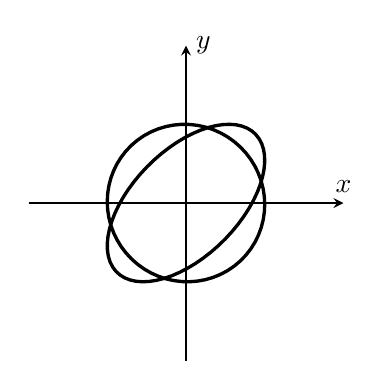
\begin{tikzpicture}
  \tikzmath{
    \a = 2;
    \b = 3;
  }
    \draw[->,>=stealth,semithick] (-2,0)--(2,0)node[above]{$x$}; %x軸
    \draw[->,>=stealth,semithick] (0,-2)--(0,2)node[right]{$y$}; %y軸
    \draw[very thick,samples=100,domain=0:10,variable=\t] plot({sin(\a\t r)},{cos(\b\t r)});
    \draw[very thick,samples=100,domain=-10:0,variable=\t] plot({sin(\a\t r)},{cos(\b\t r)});
\end{tikzpicture}

\end{document}
